%-----------------------------------------------------------------------------------
%	PACKAGES AND OTHER DOCUMENT CONFIGURATIONS
%----------------------------------------------------------------------------------

\documentclass[11pt]{article}

\usepackage[top=2cm, bottom=3cm, left=2cm, right=2cm]{geometry}
\setlength{\parskip}{1em}
\setlength{\parindent}{4em}
\linespread{1.25}

\newcommand{\Var}{\mathrm{Var}}

\newcommand{\Cov}{\mathrm{Cov}}

\newcommand{\plim}{\rightarrow_{p}}

\usepackage{apacite}

\usepackage{amsmath, amsfonts}
\usepackage{graphicx}
\usepackage{pdfpages}
\usepackage{bm}
\usepackage{listings}
\usepackage{multirow,array}
\usepackage{enumerate}
\usepackage{bbm}
\usepackage{subfig}
\usepackage{bbm}

\usepackage[latin1]{inputenc}

\usepackage{amssymb}

\usepackage{mathrsfs}
\usepackage{float}
\usepackage{booktabs}
\usepackage{color}
\usepackage{rotating}
\usepackage{amsthm}
\usepackage{multirow,array}
\usepackage{caption}
\usepackage{url}



\DeclareMathOperator*{\argmax}{arg\,max}
\DeclareMathOperator*{\argmin}{arg\,min}

\usepackage{fancyhdr}

\pagestyle{fancy} % Turn on the style
 % Start with clearing everything in the header and footer
% Set the right side of the footer to be the page number
\fancyfoot[R]{\thepage}

% Expectation symbol
\newcommand{\E}{\mathrm{E}}
\newcommand{\V}{\mathrm{V}}
\newcommand{\N}{\mathcal{N}}
\newcommand{\R}{\mathbb{R}} 

%----------------------------------------------------------------------------------
%	TITLE AND AUTHOR(S)
%----------------------------------------------------------------------------------

\title{Asymmetric Learning Model of Resume Building With Wage Rigidity and Costly Firings} % The article title

\author{Nathan Mather} % The article author(s) 

\date{\today} % An optional date to appear under the author(s)

\renewcommand{\contentsname}{Table of Contents}
%----------------------------------------------------------------------------------
\begin{document}
	
	
	%------------------------------------------------------------------------------
	%	TABLE OF CONTENTS
	%------------------------------------------------------------------------------
	\maketitle % Print the title/author/date block
	
	\setcounter{tocdepth}{3} % Set the depth of the table of contents to show sections and subsections only
	\tableofcontents % Print the table of contents
	
	\newpage
	%------------------------------------------------------------------------------
	% Introduction 
	%------------------------------------------------------------------------------

	\section{Introduction}
	
	Labor market models seek to strike a balance between including realistic aspects of the labor market, while remaining parsimonious and understandable. Asymmetric learning models incorporate the realistic assumption that current employers will know more about their own employees than competing firms.  Acemoglu and Picshke lay out an extensive model of asymmetric information and show how it can explain employers paying for general training \cite{AP_1998} \cite{AP_1999}. Progress has also been made by Uta Sch�nberg in estimating to what extent this asymmetry exists in the market \cite{Sch_2007}. While Sch�nberg finds little support for asymmetric information in the market, the logic and anecdotal evidence supporting this assumption seem strong enough to warrant additional investigation. Rather than working to empirically measure the level of asymetric information, I build out a model of asymmetric information with additional realistic assumptions about labor markets. The goal is to create a more realistic model
	
	
	The main idea and focus of my model is to investigate how wages are related to tenure in an asymmetric learning environment where outside firms only observe a resume like signal. The two period version of my model has a lot in common with the two period Acemoglu and Picshke model of asymmetric learning and general training \cite{AP_1998}. I, however, am not focusing on training, and differ from there set up in some key ways. \par
	
	NEED EDITING 
	Employers in my model will only observe a noisy signal of worker ability. In the two period model this is essentially indistinguishable from learning the true type. A firm that receives a good signal will consider that worker to have a high \textit{expected} ability rather than simply knowing they have high ability. I believe this departure will have more significant implications in a 3 period or more model. The second difference from the Acemoglu and Picshke model is that I assume outside firms can observe an employees resume. That is,  they can tell after period one if a worker was fired or separated from their firm, or if the firm decided to keep them. This has implications for the two period model, and will allow for a more realistic framework for labor force signals in 3 or more periods. Finally, I consider the impact of sticky wages and costly firings.  \par 

	
	NEED EDITING 
	The results of the model so far suggest that in an otherwise frictionless market, asymmetric information of this type will tend to lower wages and increase wage dispersion with tenure. A market with asymmetric information and sticky wages, but with high fixed costs to firing, will see relatively constant and even wages over tenure. Finally, a market with wage rigidity but moderate costs to firing will see wage growth with tenure and wage cuts for fired workers. 



%----------------------------------------------------------------------------------
% Two period Model Basics 
%----------------------------------------------------------------------------------


	\section{ Two period Model}
	
	\subsection{outline}
	
	We start by laying out the basic structure of the model. Then we consider a model without wage rigidity. We then consider what happens to this model if we introduce wage rigidity, but have no firing costs. Finally, we consider what happens as the cost to firing is increased. While the initial model without wage rigidity or firing costs closely matches a simplified version of the  Acemoglu and Picshke mode, explicitly laying out the implications of the model in this setting makes the impact of wage rigidity and firing costs more clear \cite{AP_1998} \cite{AP_1999}.
	
	\subsection{Environment}
	
	This model lasts for two periods. In the first period no firm has any information abut individual workers. The following information about the distribution of workers is common knowledge to all firms. Workers have ability $\theta \in [0,1]$ with distribution $f(\theta)$. They produce $\theta$ per period and supply labor inelastically. They take the highest wage offer they receive, and in the event of a tie stay with their current employer or pick randomly if unemployed.\par
	
	In the second period a fraction $\delta$ of workers exogenously separate from their firm. We assume that employers cannot distinguish between someone who was fired or exogenously separate. This means there is only one wage offer for all unemployed workers in period 2 with one period of experience. Employers can still offer different wages to a worker who is still employed. For workers that do not seperate, firms receive a noisy signal about employee's ability. Workers with a ability $\theta$ send a good signal with probability $\theta$ and a bad signal with probability $1-\theta$. This exact specification is not important, we just need that higher ability implies a higher probability of sending a good signal. Firms then choose whether to fire employees for a fixed cost $F_C$. Employers then offer wages to their employees for period 2 conditional on this signal. Employers offer wages to ourside workers conditional on employment history. This is because outside firms observe employee's resume, if they are employed or not, but no other signal about their ability. Workers decide where to work and produce for one more period before retiring. There are many competitive firms so this implies a zero profit condition on all firms. \par 
	
	The variables I will be using are summarized in the table below. 
	
	\begin{center}
		\resizebox{.75\linewidth}{!}{\begin{tabular}{||c | c||} 
				\hline
				Variable & Meaning  \\ [0.5ex] 
				\hline\hline
				$\theta$ & Ability \\ 
				\hline 
				$g$ & Good Signal\\ 
				\hline
				$b$ & Bad Signal \\
				\hline
				$e$ & Employed Signal\\
				\hline
				$f$ & Fired Signal\\
				\hline
				$F_C$ &  Fixed Cost to Firing \\ 
				\hline
				$\delta$ & Exogenous separation rate \\ 
				\hline
				$w_1$ &  Period 1 Wage \\ 
				\hline
				$w_g$ & Wage After Good Signal \\
				\hline
				$w_b$ & Wage After Bad Signal \\
				\hline
				$w_e$ & Wage Offered to Worker With a Year of Employment\\
				\hline
				$w_u$ & Wage for unemployed worker\\	\hline
				$\pi$ & Profits\\[1ex] 
				\hline
			\end{tabular}
		}
	\end{center}
	
The time-line is also laid out below.

	\begin{enumerate}
	\setlength{\itemsep}{1mm}
	\item period 1 wage offers
	\item Workers produce output
	\item Workers Exogenously separate
	\item Workers send signal of ability 
	\item Employers decide who to fire
	\item Employers offer period 2 wages conditional on signal. That is $w_g$, and $w_b$
	\item Outside Firms offer wages conditional on resume. That is $w_e$, and $w_u$
	\item Workers take the best offer and work for one more period 
	\item Workers retire 
\end{enumerate}



%----------------------------------------------------------------------------------
% Flexible Wage Model
%----------------------------------------------------------------------------------


\subsection{Flexible Wage Model}

First we will consider a model with totally flexible wages. In this model there is no reason to ever fire workers. Employers can simply lower wages to whatever level is profitable or induce a worker to quit. Note that in period 2 the expected output of employees who sent a good or bad signal is $\E[\theta|g]$ and $\E[\theta|b]$ respectively. 

\textbf{Proposition 1:} Second period wages in the flexible model will be $w_g = \E[\theta|g]$,  $w_b = \E[\theta|b]$, and  $ w_u =  \frac{ \delta \E[\theta] + (1-\delta)p(b)( \E[\theta | b])}{\delta + (1-\delta)p(b)}$. All Workers who send a bad signal will quit and switch firms. 

To determine wages we use backward induction and begin in the second period. To start, let's remain agnostic about who will quit after the first period. Let $Q$ denote the fraction of workers that don't separate and then quit. We know the wage offer to an unemployed worker given $Q$ is 

 $$ w_u(Q) = (\delta \E[\theta] + Q \E[\theta | \text{worker quit}])/(\delta + Q)$$
 
We also know that employers will not pay their low signal employees more than $\E[\theta | b]$ since this would result in a loss. They also cannot pay them less since an outside employer would pay at least $\E[\theta | b]$ for any worker. This implies 

 $$ w_b = \E[\theta | b] $$
 
 Using these two equations we can show the following lemma
 
 \textbf{Lemma 1:}  $w_u > w_b$
 
 The lowest possible $w_u$ is if the pool of workers has the lowest average skill. That is, if all bad signal employees quit and no good signal employees quit. This gives us
 
 $$\E[\theta|b] < \min w_u(Q) = \frac{ \delta \E[\theta] + (1-\delta)p(b)( \E[\theta | b])}{\delta + (1-\delta)p(b)} $$
 
 Lemma 1 implies that all bad signal employees will quit to receive $w_u$ rather than $w_b$. If all bad signal employees quit, than any worker who is still employed after period 1 must be high skill, which implies 
 
 $$ w_e = w_g = \E[\theta|g]$$
 
 Since this is the outside offer for employed workers. Quitting would mean workers enter a pool with some low signal employees and take a wage cut, so high signal employees do not quit. 

\textbf{proposition 2:} First period wages in the flexible model will be $$w_1 = \E[\theta]$$

Given the wages in period 2, in order to determine period one wages all we need to do is apply the zero profit condition. The period one wage will be equal to period one output plus expected profits in period two. Only good workers are retained and employers earn zero profits on them, so first period wages are just the expected output in the first period. 
 
 Putting this together we get $ w_g >w_1 > w_u $. That is, over time wages increase on average for good workers and decrease on average for bad workers increasing the spread of wages over time. Additionally, we get from this model that any workers who are sending bad signals to their employers will just quit rather than face wage cuts. This matches some intuition about the labor market but it also seems unrealistic because large real wage cuts don't typically happen. Moreover, if an employer is dissatisfied with an employee they are likely to fire them, not cut their wage an induce them to quit.In fact, in the above model no one is ever fired, and with the ability to countlessly lower wages the existence of any firings don't really make sense. To correct this I first introduce sticky wages. \par 
 
 
 
 %----------------------------------------------------------------------------------
 % sticky wages, no firing costs 
 %----------------------------------------------------------------------------------
 
 
 \subsection{ sticky wages with no firing costs }
 
 In this section we introduce downward wage rigidity or "stick wages" into the model. By ``downward wage rigidity" I explicitly mean that firms cannot cut wages in period 2 from what they were in period 1. We will also start by assuming that the fixed cost to firing employees, $F_C$, is zero. 
 
  \textbf{proposition 4:} Wages in an equilibrium with no firing costs and sticky wages are  $w_1 = \E[\theta]$,  $w_g = \E[\theta|g]$,  $w_b = \E[\theta|b]$, and  $ w_u =  \frac{ \delta \E[\theta] + (1-\delta)p(b)( \E[\theta | b])}{\delta + (1-\delta)p(b)}$. The same as without sticky wages.
 
 
 To solve this problem we will again want to use backward induction. However, we now need to know which wages in the second period are stuck, i.e. equal to $w_1$. For this, it seems, we need to know $w_1$ first, creating a problem for backward induction. This could be solved by simply checking each possibility for an equilibrium, but we we can instead determine which wages are stuck using the zero profit condition. 

We know that $w_1 \in \Big(\E[\theta|b], \E[\theta|g] \Big)$. This is because We know that the profit maximizing wage offers, without wage rigidity, for firms in period 2 will be the wages offered in the flexible mode. So, if the firm offers period one wages 
$w_1 \leq \E[\theta | b]$ they can offer the same wages as in the flexible model in period two 
and receive positive profits. This does not satisfy the zero profit condition and so will not be an equilibrium. If a firm offers first period wages $w_1 \geq \E[\theta|g]$ they will not be able to lower wages in the second period. They will be paying wages higher than the maximum output and so clearly earn negative profits. Thus, this is also not an equilibrium. \par 

The above fact implies  $w_b = w_1$ because $w_b$ will be ``stuck". So, since firing is costless, firms will fire low signal employees. Since only high signal employees are left employed we get the same outcome as in the flexible wage scenario (proposition 4). Except now bad signal employees are fired rather than quiting. 
 
 
 
 %----------------------------------------------------------------------------------
 % sticky wages and firing costs 
 %----------------------------------------------------------------------------------
 
 \subsection{sticky wages and firing costs }
 
 
	%----------------------------------------------------------------------------------
	% low firing costs 
	%----------------------------------------------------------------------------------
 
	 \subsubsection{Low firing costs}
	 
	 NEEDS EDITING. The sticky wage result of all bad signal workers being fired at lest acknowledges the existence of firing, but it may not be completely satisfactory either. Certainly employers don't fire employees as soon as their expected output drops just below their wage? Firing employees and creating turnover can be difficult.  Some firms may face extremely high fixed costs to firing through legal risk, difficulty building a case for firing workers, difficulty getting managers to fire employees, or strong unions. (ADD SOME EXAMPLES AND SOURCE)\par 
	 
	 next we incorporate a fixed cost to firing employees. If the fixed cost is very low, it will not alter the employer's behavior in period two compared to the model above with zero firing costs. They simply pay the fixed cost and fire their bad signal employees. However, this does alter the period one wage offer. Now that hiring an employee means I may have to pay a cost to fire them, their marginal benefit is decreased and so their wage offer is lower. Specifically we get
	 
	 $$ w_1 = \E[\theta] - (1- \delta)p(b)F_C$$
	 
	 
	 These wages will be a stable equilibrium whenever firms cannot deviate and receive positive profits. If a firm deviates and keeps their bad signal employees they will haveto pay them $w_1$ (because of stcky wages). These workers will not leave for another firm because leaving would identify them as a low skilled worker and yield them $\E[\theta|b] < w_1$. Therefore keeping bad signal employees gives 
	 
	 $$\pi_{keep} = \E[\theta] - w1 + (1-\delta) \Big(p(g)(\E[\theta|g] - w_g) + p(b)(\E[\theta|b] - w_1 )\Big) = \E[\theta] - w_1 +  (1-\delta) \Big( p(b)(\E[\theta|b] - w_1) \Big) $$
	 
	 compared to firing them and receiving 
	 $$\pi_{fire} = \E[\theta] - w1 + (1-\delta) \Big( p(g)(\E[\theta|g] - w_g) - p(b)F_C \Big) $$
	 
	 and so firing workers is optimal for all firms as long as the fixed cost to firing is less than the loss from holding onto a bad signal worker.
	 
	 $$ w_1 - \E[\theta|b] > F_C$$
	 
	  $$ \implies  \E[\theta] + (1- \delta)p(b)F_C -  \E[\theta|b] > F_C $$
	 
	 $$ \implies f_C < \frac{\E[\theta] -  \E[\theta|b]}{1 + p(b)(1-\delta)} $$
	 
	 
	
	 This equilibrium implies $w_f < w_1 < \E[\theta] < w_g$. The intuition here is that in period two firms either make 0 expected profits on good signal workers or have to pay to fire bad signal workers. Given this, workers in the first period are paid below their expected first period output.
	 
	 
	 %----------------------------------------------------------------------------------
	 % Wage rigidity with High firing Costs 
	 %----------------------------------------------------------------------------------
		 
	 \subsubsection{High firing Costs  }
	 
	While in many cases the fixed costs to firing may be small, as in the case above, in other markets the costs may be extremely high. For example markets with extremely strong unions may make it very costly to fire a worker. Even incredibly strong worker solidarity may mean the firm incurs costs through lower productivity of current workers. If the fixed costs become sufficiently large, it is clear that firms will not fire any employees. We now explore this extreme case below. \par
	
	Given that no employees are fired, we now need to determine what equilibrium wages will be when firms retain both high and low signal workers. It is also clear from the above work that $w_b = w_1$ since those wages are stuck. This also implies $w_b \leq w_g$. 
	
	 When considering what to offer a worker who is currently employed and a different firm, $w_e$, all a firm knows is the general distribution of worker types. So they can infer $\E[\theta|e]$. We can start by noting that firms will always offer $w_e \leq \E[\theta|e]$. This is because if firms offer $w_e$ such that $ w_b < w_g \leq \E[\theta | e] < w_e$ outside firms get all workers but at an expected loss. \par 
	 
	 Next, consider the case where $\E[\theta|b] \geq w_b < w_e < w_g$ outside firms only attract bad signal employees for a negative expected profit so this cannot be an equilibrium. Finally if $ w_e \leq w_b \leq w_g \leq \E[\theta | e]$ the outside offer attracts no workers and so outside firms earn zero profits. If they ahve an incentive to deviate depends both on $w_g$ and assumptions about the structure of the market. 
	
	 Acemoglu and Picshke assume that current employers can always move second and get the last offer in. This leads to a "winners curse" that would keep outside offers low even if $w_g < \E[\theta|e]$ \cite{AP_1998}. In this outcome  $ w_e \leq w_b = w_g = w_1$.  I, however, work on the assumption that employers must set their wages first then outside firms make their offers. While the former way matches the framework of, for example, the academic market, where countering outside offers is popular, my logic more closely matches many typical labor settings. Employers have wages set and can not validate outside offers. If an employee gets a better offer elsewhere employers often simply let the employee go. Under these assumptions we get  $w_1 + \epsilon < \E[\theta|e]$ for a positive profit on all workers. In this framework a stable outcome is $w_b = w_1$, and $w_g = \E[\theta|e]$. With these wage offers any offer an outside firm makes will result in a loss and so they simply offer a wage low enough to attract no workers, $w_e = \E[\theta | b]$. \par 
	
	This gives us 
	
	$$ w_g = E[\theta | e] =\E[\theta]$$
	
	They will pay their bad signal employees as little as possible 
	$$ w_b = w_1$$ 
	
	unemployed workers get their expected output 
	$$ w_u = E[\theta] $$
	
	this gives a first period wage through the zero profit condition 
	$$w_1 = \E[\theta] + (1-\delta)(p(g)(\E[\theta|g] - \E[\theta]) + p(b)(\E[\theta|b] - w_1))$$
	
	
	using the fact that $p(g)\E[\theta|g] + p(b)\E[\theta|b] = \E[\theta]$ we get 
	
	$$ w_1 = \E[\theta] +  (1-\delta)(\E[\theta] - p(g)\E[\theta] - p(b)w_1)$$
	
	using the fact that $ \E[\theta] - p(g)\E[\theta] = p(b)\E[\theta]$
	
	$$ \implies  w_1 = \E[\theta] +  (1-\delta)p(b)(\E[\theta] - w_1) $$
	$$ \implies w_1 +(1-\delta)p(b)w_1 = \E[\theta] + (1-\delta)p(b)\E[\theta]$$
	
	$$ \implies w_1 = \E[\theta]$$
	
	So all workers get paid $\E[theta]$ no one is fired and also no workers are induced to quit since quiting gets them the same wage. Firms have inside information but they are too restricted to do anything with it. They can't lower their bad employees wages or fire them. \par 
	
	This equilibrium will be stable whenever it is more costly to fire an employee then to keep them at this wage. That is when 
	
	$$ F_C >  w_1 - \E[\theta|b] = \E[\theta] - \E[\theta|b]$$
	
	The implication of this is that sticky wages make it impossible for firms to capitalize on their inside information in period 2 by cutting worker's wages while the high firing costs are making it impossible to use inside information for strategic firing. Thus, they earn no profits in period two and incur no costs; So period one wages are not bid up past expected revenue in period 1.
	
 	While I find this story fairly conniving, there is some aspect of firm behavior that still doesn't seem quite right to me. Specifically wages are treated exogenously in the stability condition. In a later section we explore the possibility of an extension to the model that allows wage offers specific to each firm that would make wages endogenous to firm's decisions about firing employees. This extension would clear up much of the logic above and make the model more accurate, albeit much more complicated. 

	 
	 
		 
	 
	 %----------------------------------------------------------------------------------
	 % Mixed Equilibrium
	 %----------------------------------------------------------------------------------
	 
	\subsubsection{Mixed Equilibrium}
	
	
	Now consider the case between the two extremes outlines above. That is, whenever 
	
	$$ F_C \in \left[  \frac{\E[\theta] - \E[\theta]}{1 + p(b)(1-\delta)} , \E[\theta] - \E[\theta|b] \right] $$
	
	In this case employers will fire a fraction of their bad signal workers $\delta_F$ until they are indifferent between firing and keeping them 
	$$  F_C = w_1 - E[\theta|b]$$ 
	
	Good signal employees need to be paid the expected output of an average worker employee in period 2, for the same reason outlined in the section above. This gives us
	
	$$ w_g(\delta_F) = \frac{p(g)\E[\theta|g] + p(b)(1-\delta_F) \E[\theta|b] }{p(g) + p(b)(1-\delta_F)} $$
	
	bad signal employees are paid the lowest wage possible $ w_b = w_1$ and unemployed get their expected output 
	
	$$ w_u = \frac{ \delta\E[\theta] + (1-\delta) p(b) \delta_F \E[\theta | b]}{  \delta + (1-\delta) p(b)\delta_F} $$
	
	by the zero profit condition we get the first period wages 
	
	$$w_1 = \E[\theta] + (1-\delta)  \bigg( p(g) \Big(\E[\theta|g] - w_g(\delta_F)  \Big) - p(b)F_C  \bigg) $$

	
	Given an exogenous separation rate, we can also calculate the fraction of workers fired $delta_f$.  We have two equations for $w_1$ with the only unknown being $\delta_F$. I have solved for it below, but it not very intuitive. We can see that as the fixed cost rises the fraction of workers fall. It can also be used to solve numeric examples.
	

		
		\newcommand{\TAMEG}{\frac{\E[\theta] -  (1+(1-\delta)p(b))F_C - \E[\theta|b]}{(1-\delta)p(g)}}
		
		$$ \delta_F = \frac{p(g) \left[\TAMEG \right]}{ p(b) \left[ \E[\theta | b] - \TAMEG - \E[\theta|g] \right] } $$
		
	


%----------------------------------------------------------------------------------
% Numerical examples 
%----------------------------------------------------------------------------------

\section{Numerical Examples}


While the above work characterizes the equilibrium for any set of parameters, in order to visualize the impact that fixed costs and separation rates have on wages we graph a numerical example. Theta is distributed uniformly from 0 to 1 \footnote{This is discretized over 100 points in order to calulate it all in R}. We then plot the wages for each group for 200 fixed costs evenly distributed between 0 and 0.25. We stop at 0.25 because after this all wages are 0.5 and no one is fired. We do this for separation rates $\delta$ of .2, .4, .6, and .8. The results are in figure 3. \par 

First we see that wages for unemployed workers start low with a low fixed costs, since the pool of workers is filled with bad signal workers who are fired. After fixed costs reach the point where not all bad signal workers are fired, unemployed wages move up until no one is fired. A higher exogenous seperation rate means higher unemployed wages because there are more average workers to dilute the pool of bad fired workers. \par 

Period 1 wages decline immediately with fixed costs as employers pay the fixed costs to fire bad employees. Eventually, however, employers stop firing all their bad signal employees and thus are paying lower fixed costs and earning profits on high signal workers which raises period one wages until they return to 0.5 where no one is fired. \par 

Bad signal workers who are  fired simply track unemployed wages until bad signal workers are no longer fired. Bad signal workers who are not fired just track period 1 wages since their wages are stuck. \par 

Finally, good signal wages start out high. Since bad signal workers are fired and so being employed is a signal of high ability. However, as firms start retaining some of their bad signal employees they are able to underpay their good signal employees and take advantage of their inside information. 


\begin{figure}[H]
	\centering
	\LARGE{\textbf{Figure 3}}
	\subfloat{		
		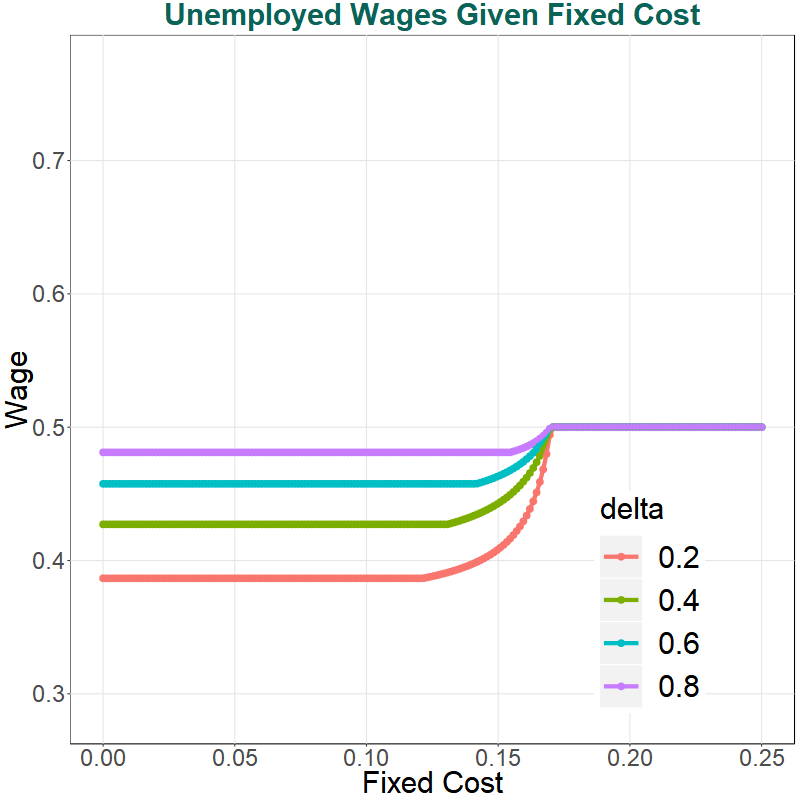
\includegraphics[width=.45\linewidth]{Unemployed_Wages_Given_Fixed_Cost.png}
	}
	\subfloat{
		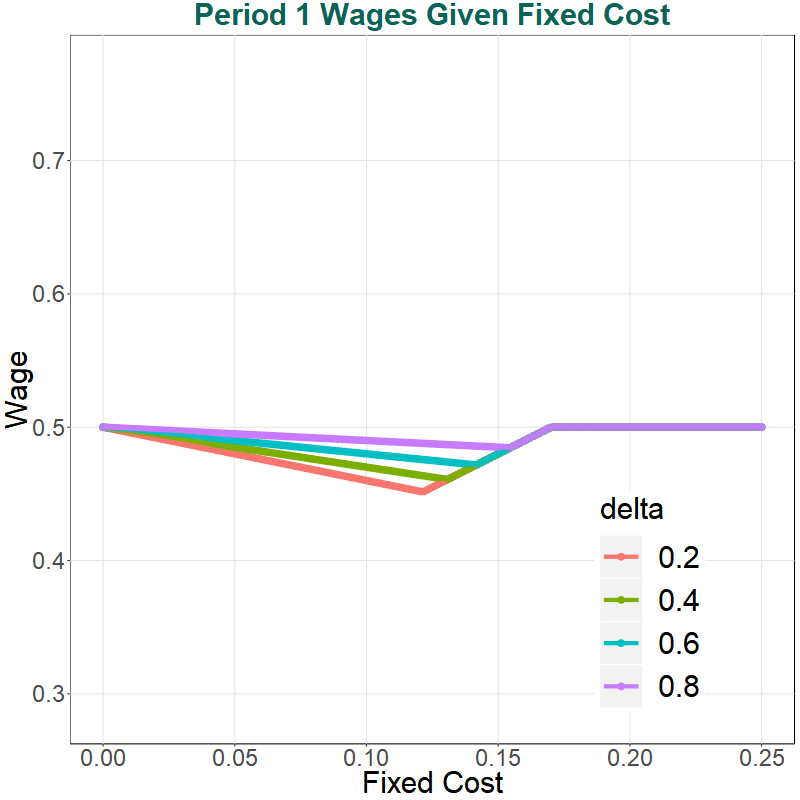
\includegraphics[width=.45\linewidth]{Period_1_Wages_Given_Fixed_Cost.png}
	}
	\newline
	\subfloat{
	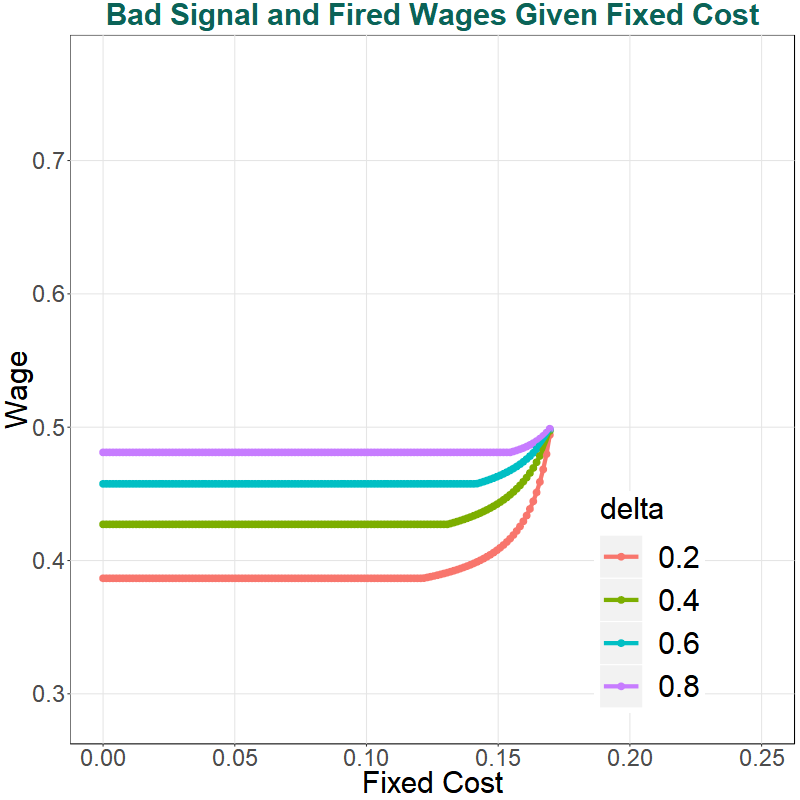
\includegraphics[width=.45\linewidth]{Bad_signal_and_fired_Wages_Given_Fixed_Cost.png}
	}
	\subfloat{
		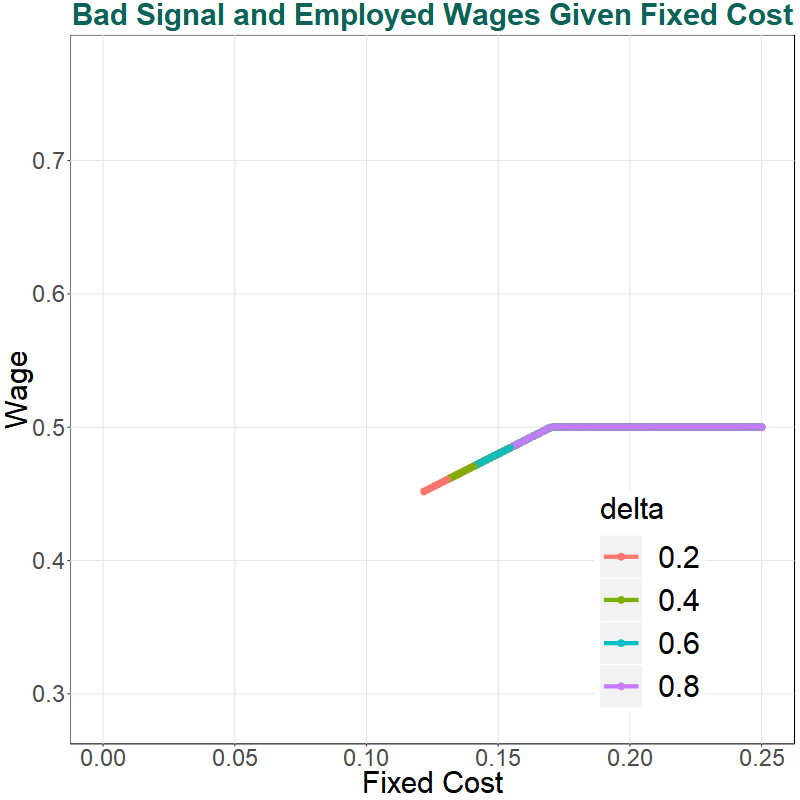
\includegraphics[width=.45\linewidth]{Bad_signal_and_employed_Wages_Given_Fixed_Cost.png}
	}
\newline
	\subfloat{
	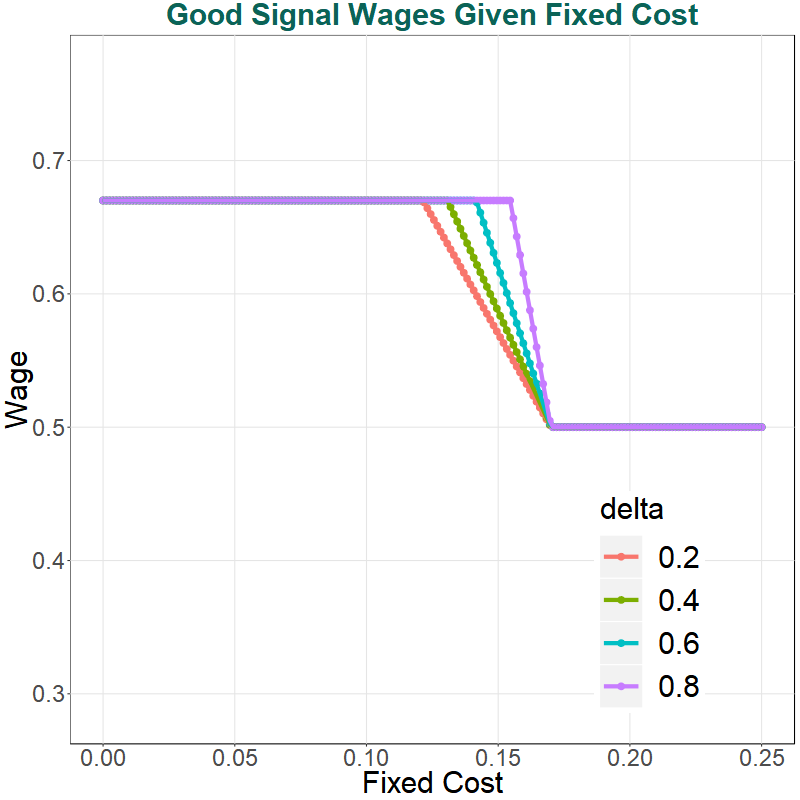
\includegraphics[width=.45\linewidth]{Good_Signal_Wages_Given_Fixed_Cost.png}
	}

	
\end{figure}

%----------------------------------------------------------------------------------
% Future Work
%----------------------------------------------------------------------------------

\section{Future work}

While I have learned a lot from working on this project, there are still many aspects of this model to consider more closely and expand upon. The most crucial area to take a closer looks is at my implicit assumption that all firms offer the same wages $w_g$ and $w_b$ after good an bad signals. This leads to a more shaky definition of a mixed equilibrium than I would like. While firms don't have additional information about other firms workers, they do know the composition of good and bad signal workers in their own firm in period two. It does make more sense that firms . While I have not had time to fully work out the math on this realization, my initial investigation is suggesting that this adds significant complexity to the problem. 

This introduces another element to the problem in which each firm needs to consider the benefit of holding onto bad signal workers in order to hide information from outside firms and underpay their good workers. 

This is all dependent on the size of the firm and their distribution of workers as well as period 1 wages since their bad employees will need to be paid this wage. 



\section{Conclusion}
Overall the model makes generally unsurprising predictions about wages in the . 

Some interesting predicitons are the trend in period one wages as fixe costs rise and the heterogenous impact of exogenous seperation given various fixed costs. 

That being said, there is certainly room for improvident in the formulaton of the model and in how a similar motivation and defining characteristics could be used. 


%------------------------------------------------------------------------------
% bib
%------------------------------------------------------------------------------


\bibliographystyle{apacite}
\bibliography{References}
	
	%------------------------------------------------
	% end doc
	%------------------------------------------------
\end{document}





